\documentclass[12pt]{article}
\usepackage{graphicx}
\usepackage{wrapfig}
\usepackage{subfigure}
\usepackage{multirow}
\usepackage{hyperref}
\usepackage{amsmath}
\usepackage{amssymb}
%\usepackage{ngerman}
\usepackage[ansinew]{inputenc}
\usepackage[left=2cm,top=1cm]{geometry}

% vector graphics test
\usepackage{color}
\usepackage{transparent}
\graphicspath{{graphs/}}

\setlength{\parindent}{0pt}

%\usepackage[outdir=./]{epstopdf}
%\epstopdfsetup{outdir=./}


\begin{document}
	\pagestyle{empty}
	

\begin{titlepage}
	\centering
	\bigskip
	\huge{Astronomisches Praktikum:\\Spektrale Klassifikation extragalaktischer Objekte}\\
	\bigskip
	\large{Versuch 10}\\
	\bigskip
	\large{Jan R\"{o}der \& Julia Lienert}
	\bigskip
	\tableofcontents
\end{titlepage}

\pagebreak


\section{Einleitung}



\section{Spektrografie}

\subsection{Aufgabe 1}

\begin{figure} [h]
	\centering
	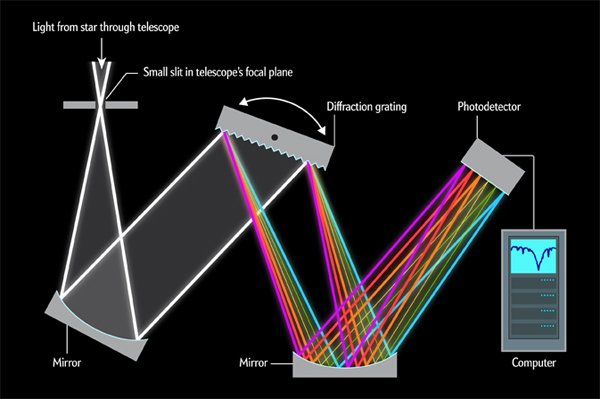
\includegraphics[width=0.8\textwidth]{spectrograph.jpg}
	\caption{Schematischer Aufbau eines Spektrographen}
	\label{fig:spektrograf}
\end{figure}

Abbildung \ref{fig:spektrograf} zeigt den schematischen Aufbau eines Spektrographen. Licht f\"{a}llt durch das Objektiv des Teleskops, wo es durch einen Hauptspiegel auf ein Gitter projiziert wird. Dieses Gitter hat Dispersionseingenschaften, wodurch das Licht in seine Bestandteile zerlegt wird. Das Aufgespaltene Licht f\"{a}llt nun auf einen zweiten Spiegel, der das Licht gerade so auf einen Detektor reflektiert, dass die Farben ``geordnet'' dort auftreffen. Je nach Wellenl\"{a}ngenbereich kann der Detektor eines anderen Typs sein.  Die Rotationsm\"{o}glichkeit des Gitters bestimmt, welche Wellenl\"{a}ngen des einfallenden Lichts \"{u}berhaupt bis zum Detektor kommen.

\subsection{Aufgabe 2}

Eine Linie oder einen \"{U}bergang nennt man ``verboten'', wenn er im Labor nicht erzeugbar ist, er aber dennoch beobachtet wird. Oft treten diese Linien in Gasen geringer Dichte auf, wo St\"{o}sse mit anderen Molek\"{u}len unwahrscheinlich sind. Wird dann ein Gasteilchen auf ein h\"{o}heres Energieniveau gehoben, wird der \"{U}bergang zur\"{u}ck in den Grundzustand als ein verbotener \"{U}bergang erfolgen. Beispiele sind z. B. die O[III]-Linie bei etwa 500\,nm oder die 21\,cm-Linie des Wasserstoffs.


\section{Analyse eines Galaxien-Spektrums mit IRAF}

Im Datenset ist die Wellenl\"{a}nge $\lambda$ auf der x-Achse aufgetragen. 


















\section{Diskussion}




\section{Quellen}
\begin{enumerate}
	\item Versuchsanleitung zu Versuch 8: "Planetenbahnen"
	\item https://de.wikipedia.org/wiki/Parallaxe
\end{enumerate}


%\begin{figure} [h]
%	\centering
%	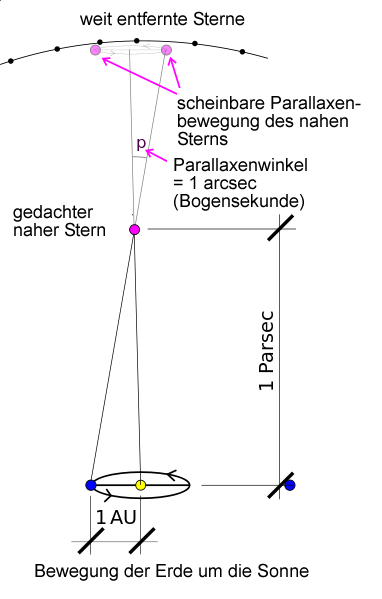
\includegraphics[width=0.4\textwidth]{2_4_Parallaxe.png}
%	\caption{Skizze zur Erkl�rung der Parallaxe (entnommen aus [2])}
%	\label{fig:Parallaxe}
%\end{figure}








\end{document}